\documentclass[a4paper,11pt,oneside,openany,brazilian,version=last,draft=false,]{main}
\usepackage[centerlast,small,sc]{caption}
\setlength{\captionmargin}{30pt}

\usepackage{graphicx}
\usepackage{natbib}        % required for bibliography
\usepackage[utf8]{inputenc}
\usepackage{mybook}
\usepackage{float}
\usepackage{fancyhdr}
\usepackage{pdfpages}
\usepackage {subcaption}
\usepackage{color}
\sloppy  


\pdfcompresslevel = 9
\oddsidemargin = 31pt
\topmargin = 20pt
\headheight = 12pt
\headsep = 25pt
\textheight = 592pt
\textwidth = 390pt
\marginparsep = 10pt
\marginparwidth = 35pt
\footskip = 30pt

\usepackage[top=1.5in, bottom=1.25in, left=0.8in, right=0.8in]{geometry}




\begin{document}



\thispagestyle{empty}

%% Restart page counter.
\setpagecounter{0}

%% Disable page anchor to avoid multiple page number definition warnings.
\hypersetup{pageanchor=false}

\vspace{4cm}

 \textcolor{gray}{Execução:} \\
\\
\begin{minipage}{\textwidth}
	\centering
       
	
\includegraphics[width=0.3\textwidth]{logos/lead-logo}
	
\end{minipage}

\vspace{2cm}

\textcolor{gray}{Financiamento: } \\ 
\\
\begin{minipage}{\textwidth}
	\centering
	
	
\includegraphics[width=0.3\textwidth]{logos/esbr-logo}
	
\includegraphics[width=0.3\textwidth]{logos/aneel-logo}

	
\end{minipage}

\vspace{4cm}

\begin{table}[ht!]
	\centering
	\begin{tabular}{r l|l p{12cm} }
		\textcolor{gray}{Projeto} &&& \textbf{\Large EMMA}\\
			&&& \textbf{Robô para Inspeção de Turbinas}\\
			&&& \\
		\textcolor{gray}{Título} &&& \textbf{Relatório de Viagem}\\
		\textcolor{gray}{PD} &&& 6631-0003/2015 \\
		\textcolor{gray}{Contrato} &&& Jirau 09-15\\
		\textcolor{gray}{Coordenador} &&& Ramon Romankevicius Costa \\
		\textcolor{gray}{Gerente} &&& Breno Bellinati de Carvalho \\
		\textcolor{gray}{Período do projeto} &&& 26.02.2015 - 26.04.2016 \\
		\textcolor{gray}{Data da viagem:} &&& 30.05.2016 - 31.05.2016 \\
	\end{tabular}
\end{table}


\cleardoublepage

%%==============================================================================
%% AUTHORS AND VERSION PAGE
%%==============================================================================
\begin{onecolumn}
\thispagestyle{empty}

%% Restart page counter.
\setpagecounter{0}

\begin{center}
  %% Version section. --------------------------------------------------------

  
 \vfill
  %% Project section. --------------------------------------------------------


  %% Authors section. --------------------------------------------------------

  \center{\LARGE Participante(s)}
  
  \vspace{0.50cm}



  \begin{center}
    \begin{tabular}{| l | l | l | l |}
    
    \hline
   	 Nome 					& Função			 & Qualificação 	& Instituição	 \\\hline
   	 Ramon Romankevicius 	& Coordenador 	 	 & DO			    & UFRJ  	\\\hline		
	 Breno Carvalho			& Gerente do Projeto & SU 			    & ESBR 		\\\hline
	 Gizelle Ferreira 		& Engenheira de P\&D & SU 				& ESBR 		\\\hline
	 Iúri Gadelha	 		& Engenheira de P\&D & SU 				& ESBR 		\\\hline
	 Darlan Geremia 		& Pesquisador		 & SU 				& Rijeza 	\\\hline
	 Jeferson Porto  		& Técnico			 & SU 				& Rijeza 	\\\hline
	  
\hline

    
    \hline 
    \end{tabular}
\end{center}

\end{center}
\end{onecolumn}

\newpage

%% Enable page anchor again.
\hypersetup{pageanchor=true}


\begin{twocolumn}

\section{Introdução}
A viagem a Jirau realizada entre os dias 30 de Maio e 31 de Maio de 2016 foi o
encerramento da primeira fase do projeto EMMA 01. 

\section{Objetivo de Viagem}
O objetivo da viagem foi
realizar a transferência de conhecimento para a equipe de operação da ESBR.


\section{Execução}
O coordenador do projeto, prof. Ramon R. Costa, apresentou a metodologia
desenvolvida no projeto EMMA e como a mesma foi alcançada.

Os tópicos abordados na apresentação foram:
\begin{itemize}
  \item Benefícios: aumento de eficiência de geração em 3-5\% a cada 30 mil
  horas, e aumento da vida útil da turbina.
  \item Objetivo: determinar a solução e metodologia para realizar o
revestimento de turbinas \textit{in situ}.
  \item Solução: manipulador industrial compacto movimentado sobre trilhos.;
  \item Metodologia.
\end{itemize}

\begin{figure}[H]
\centering
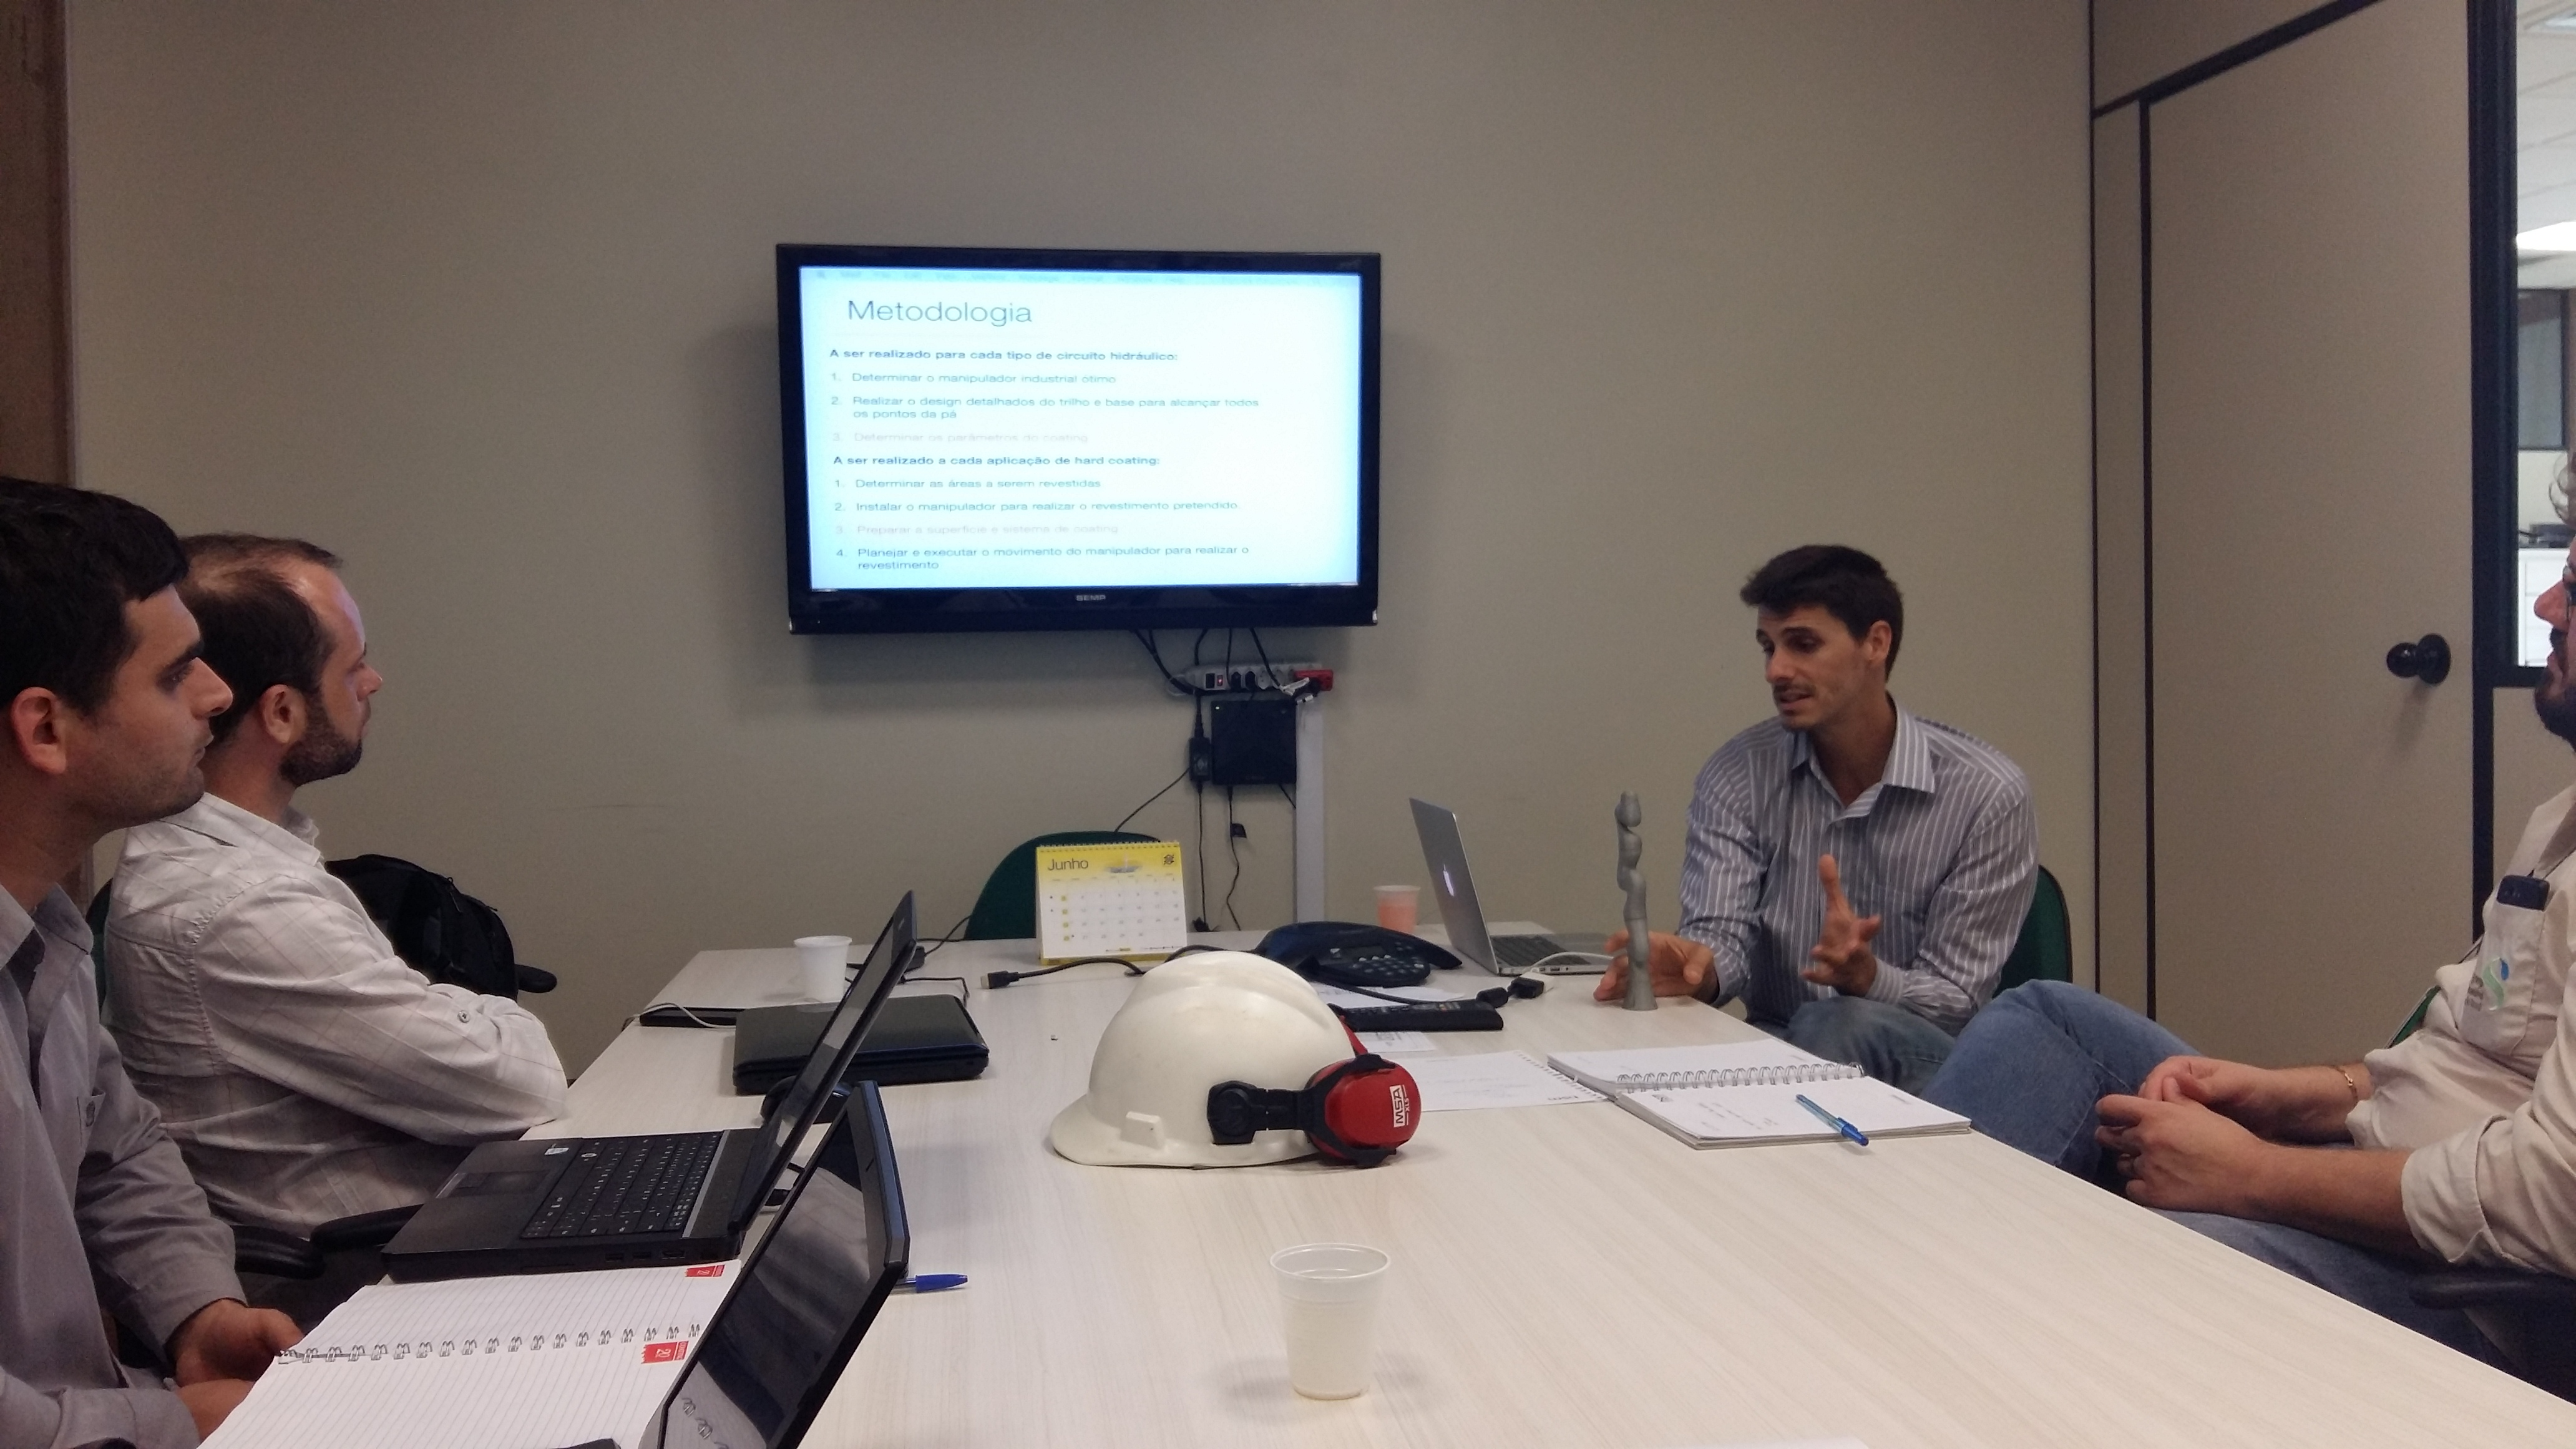
\includegraphics[width=\columnwidth]{20160530_154107}
\caption{Workshop para a transferência de conhecimento para a equipe de operação
da ESBR.}

\end{figure}

Em resumo, a metodologia foi dividida em uma análise para cada tipo de circuito
hidráulico e a análise de hard coating.

\section{Resultado}
A viagem se mostrou de grande relevância para o projeto,
uma vez que possibilitou a transferência de conhecimento adquirido durante um
ano de projeto. Foi realizada uma apresentação detalhada pelo coordenador do
projeto, Prof. Ramon Costa, destacando os benefícios, a metodologia e
esclarecendo dúvidas do projeto.
\end{twocolumn}
\end{document}
